\documentclass[12pt, onecolumn]{IEEEtran}
%\documentclass{article}
\usepackage[utf8]{inputenc}
\usepackage[T1]{fontenc}
\usepackage{lmodern}
\usepackage{graphicx}
\usepackage{color}
\usepackage{hyperref}
\usepackage{amsmath}
\usepackage{amsfonts}
\usepackage{epstopdf}
\usepackage[table]{xcolor}
\usepackage{matlab}
\usepackage{amssymb}
\usepackage{latexsym}
\usepackage{epsfig}
%\usepackage{comp}
\usepackage{algorithm}
\usepackage{algorithmic}

\begin{document}
	\author{Athar Ali (22915030)}
	\title{\bf{ \large EEN - 521 Digital Signal and Image Processing\\ Lab Report 2}}
	\maketitle 
	\markboth{\small \it{D\lowercase{epartment of} E\lowercase{lectrical} E\lowercase {ngineering}}  \hfill A\lowercase{utumn} S\lowercase{emester 
			2022} } {}
	
	%\matlabheading{EEN - 521 Digital Signal and Image Processing}
	
	
	\vspace{1em}

\begin{matlabcode}
clc
clear all
close all
\end{matlabcode}

\begin{par}
\begin{flushleft}
Solution 1:
\end{flushleft}
\end{par}

\begin{matlabcode}
%1
n=0:200;
y=10*sin(n*pi/50)+20*sin(n*pi/100);
y1=[zeros(1,50) y zeros(1,50)];
yf=movmean(y1,50);
figure; 
stem(y1);
\end{matlabcode}
\begin{center}
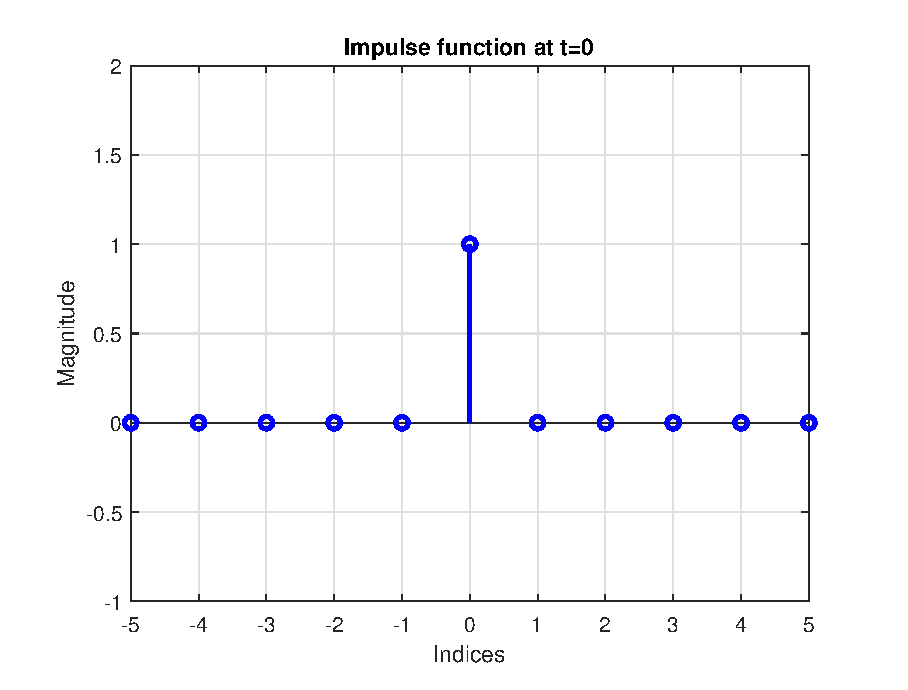
\includegraphics[width=\maxwidth{56.196688409433015em}]{figure_0.eps}
\end{center}
\begin{matlabcode}
figure; 
stem(yf);
\end{matlabcode}
\begin{center}
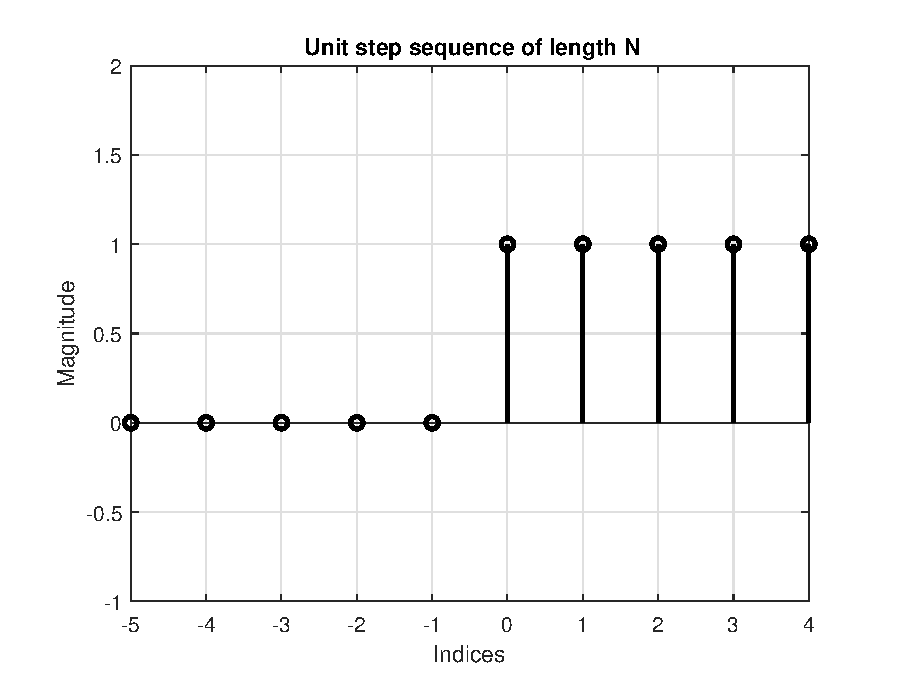
\includegraphics[width=\maxwidth{56.196688409433015em}]{figure_1.eps}
\end{center}

\begin{par}
\begin{flushleft}
Solution 2:
\end{flushleft}
\end{par}

\begin{matlabcode}
%2
n=0:50;
s=2*(n.*(0.9).^n);
figure
stem(s)
\end{matlabcode}
\begin{center}
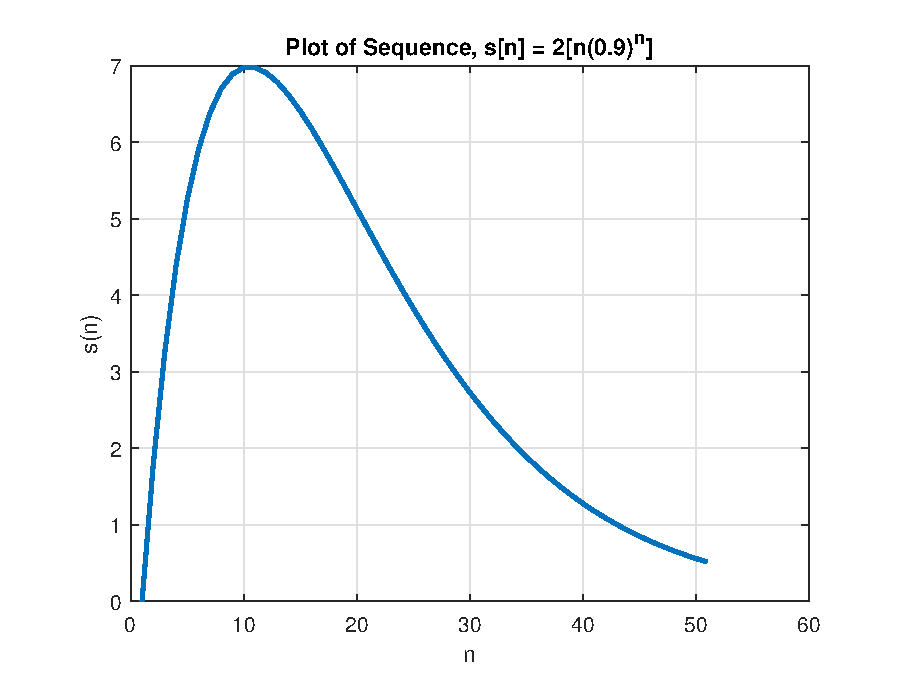
\includegraphics[width=\maxwidth{56.196688409433015em}]{figure_2.eps}
\end{center}
\begin{matlabcode}
noise=60*[n-5==0]+30*[n-7==0];
noisy=s+noise;
figure
stem(noisy)
\end{matlabcode}
\begin{center}
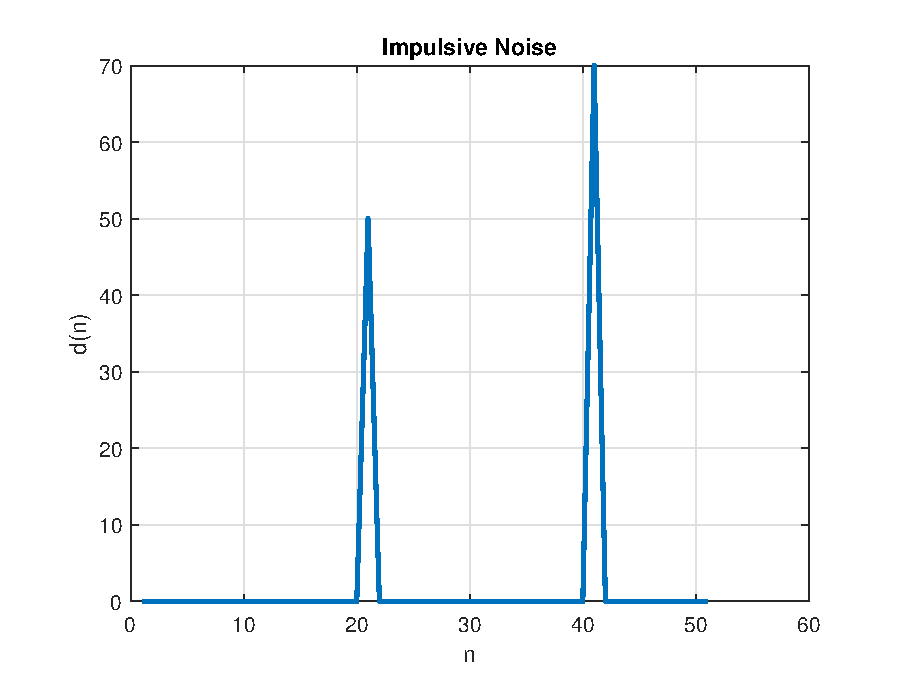
\includegraphics[width=\maxwidth{56.196688409433015em}]{figure_3.eps}
\end{center}
\begin{matlabcode}
A1=movmedian(noisy,3);
figure
stem(A1)
\end{matlabcode}
\begin{center}
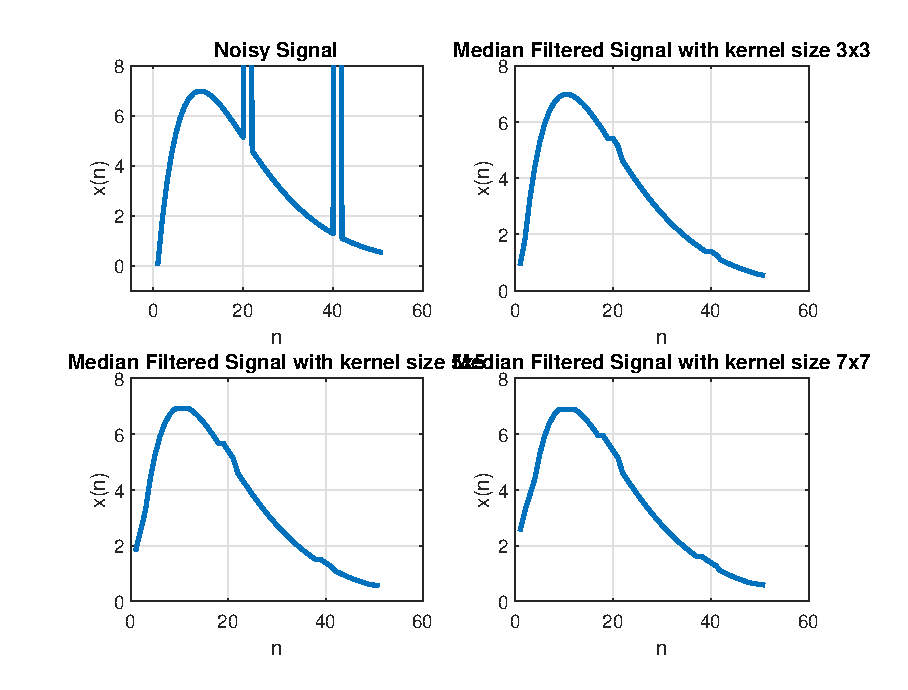
\includegraphics[width=\maxwidth{56.196688409433015em}]{figure_4.eps}
\end{center}
\begin{matlabcode}
A2=movmedian(noisy,5);
figure
stem(A2)
\end{matlabcode}
\begin{center}
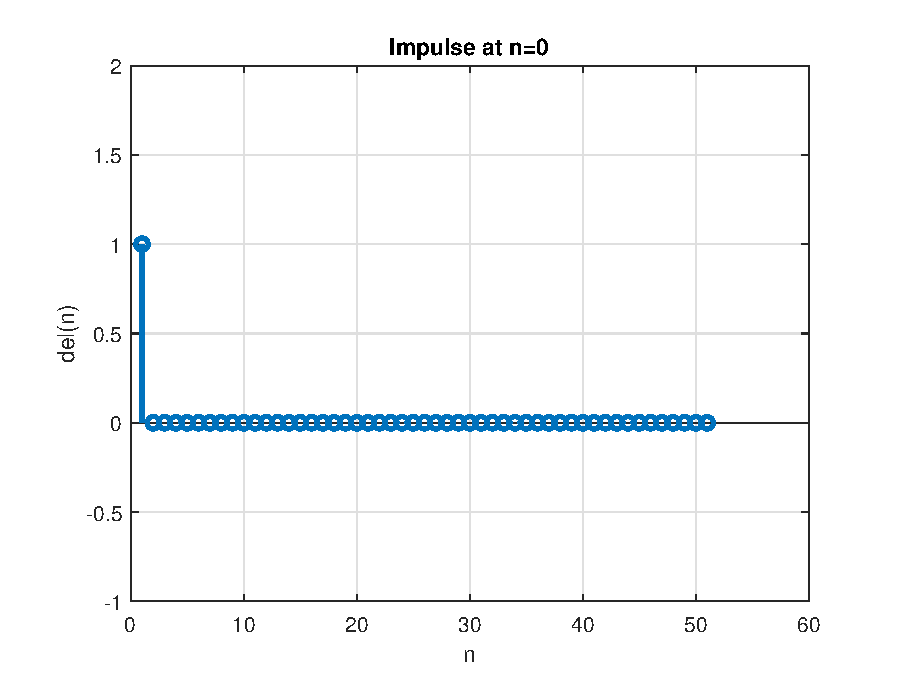
\includegraphics[width=\maxwidth{56.196688409433015em}]{figure_5.eps}
\end{center}
\begin{matlabcode}
A3=movmedian(noisy,7);
figure
stem(A3)
\end{matlabcode}
\begin{center}
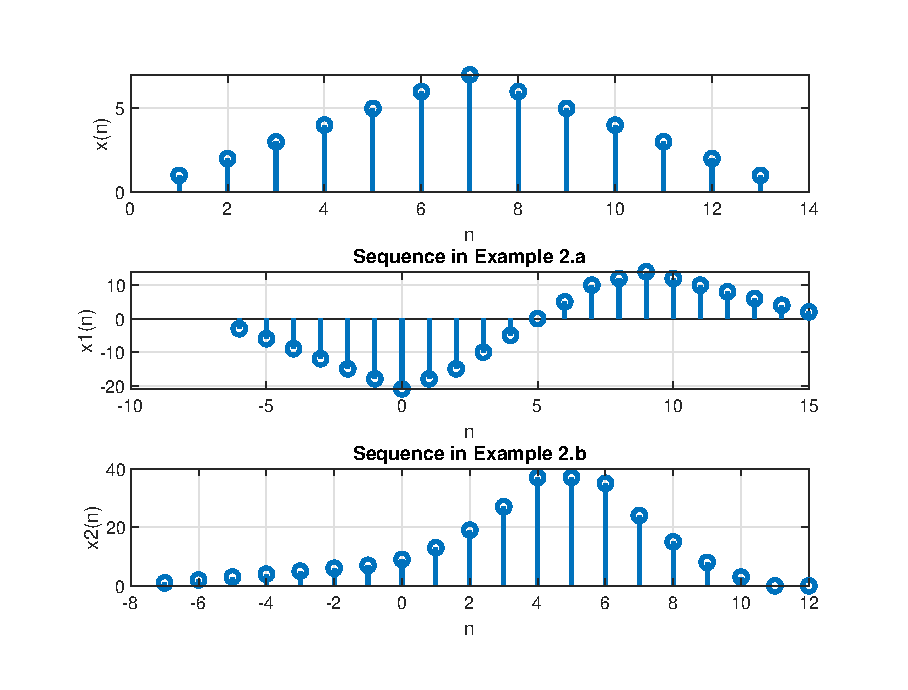
\includegraphics[width=\maxwidth{56.196688409433015em}]{figure_6.eps}
\end{center}

\begin{par}
\begin{flushleft}
Solution 3:
\end{flushleft}
\end{par}

\begin{matlabcode}
%3
n=0:50; % Indices 
b=[0.8,-0.44,0.36,0.02]; 
a=[1,0.7,-0.45,-0.6]; 
delta=[n==0]; 
Iresp=filter(b,a,delta);
units = [n>=0];
Sresp=filter(b,a,units); 
figure; 
stem(delta); 
\end{matlabcode}
\begin{center}
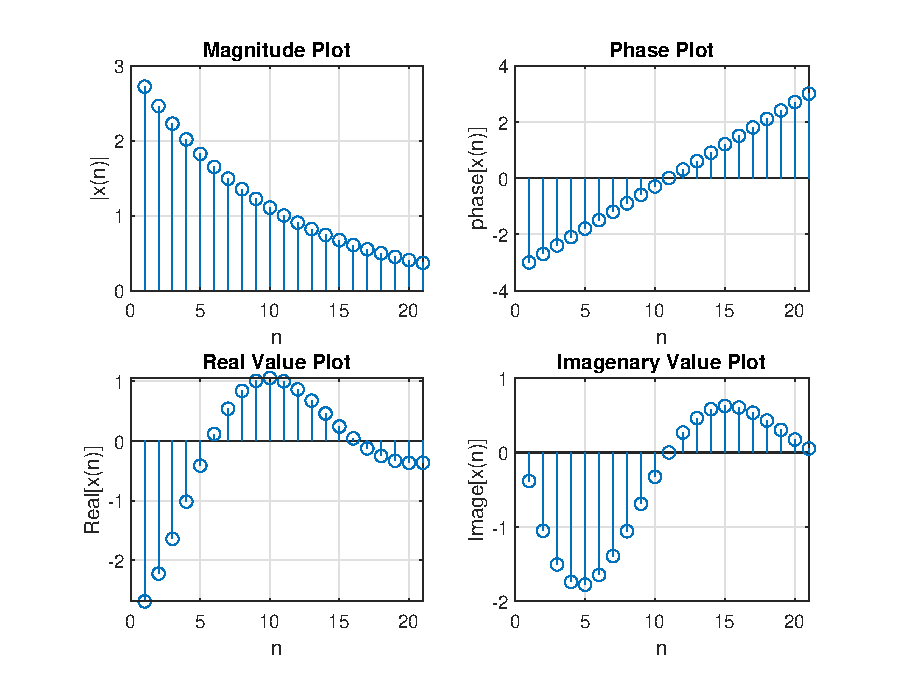
\includegraphics[width=\maxwidth{56.196688409433015em}]{figure_7.eps}
\end{center}
\begin{matlabcode}
figure;
stem(Iresp);
\end{matlabcode}
\begin{center}
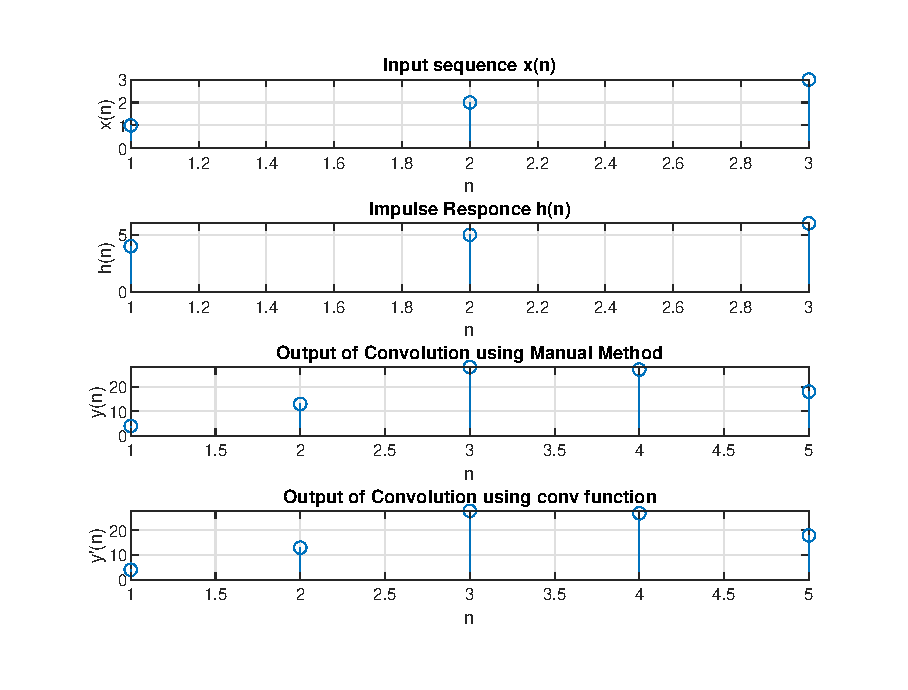
\includegraphics[width=\maxwidth{56.196688409433015em}]{figure_8.eps}
\end{center}
\begin{matlabcode}
figure; 
stem(units);
\end{matlabcode}
\begin{center}
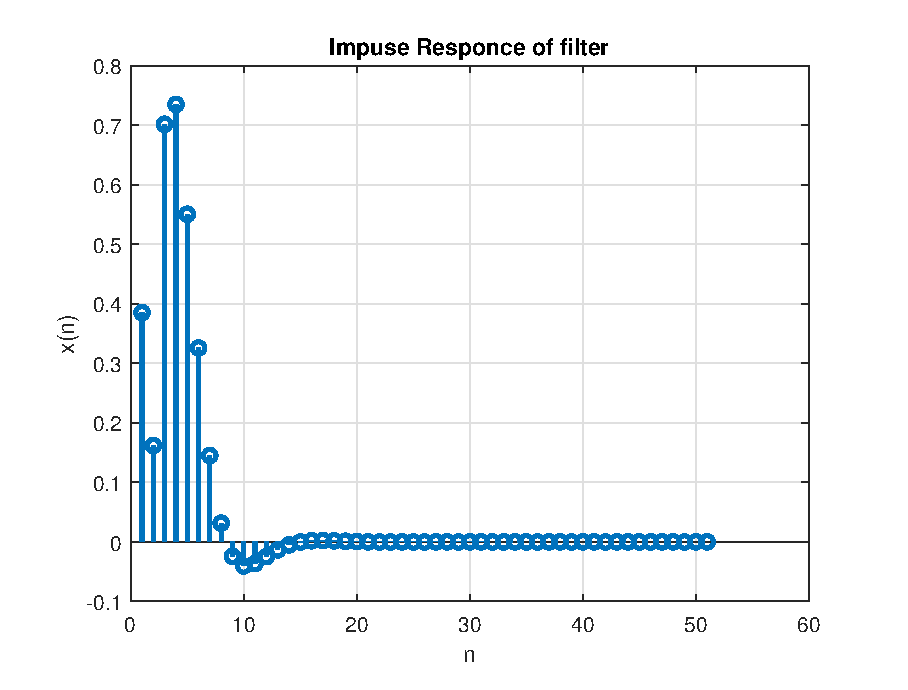
\includegraphics[width=\maxwidth{56.196688409433015em}]{figure_9.eps}
\end{center}
\begin{matlabcode}
figure; 
stem(Sresp);
\end{matlabcode}
\begin{center}
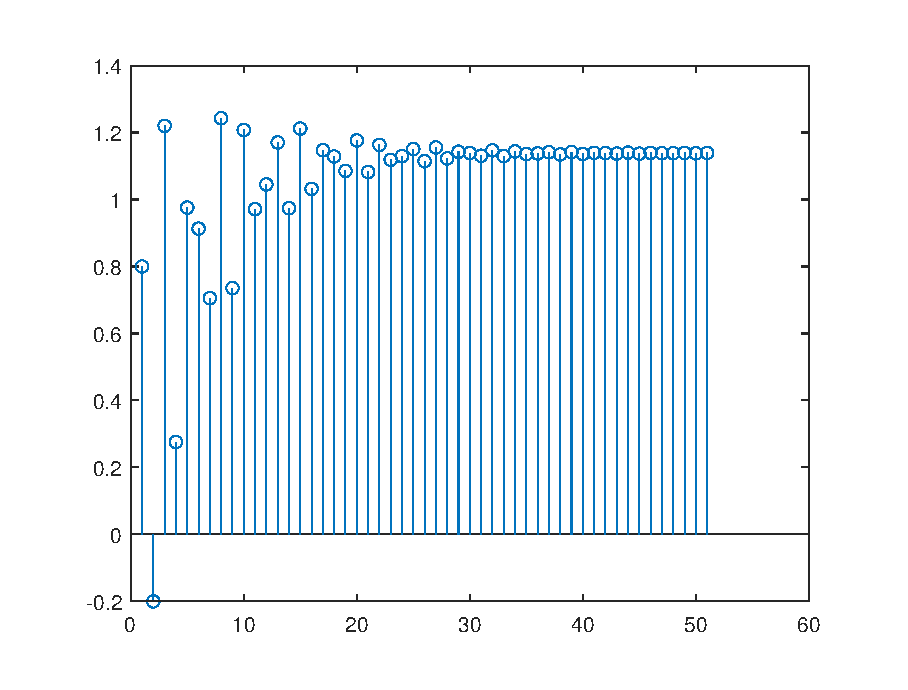
\includegraphics[width=\maxwidth{56.196688409433015em}]{figure_10.eps}
\end{center}

\begin{par}
\begin{flushleft}
Solution 4:
\end{flushleft}
\end{par}

\begin{matlabcode}
%4
b=[0.0675, 0.1349, 0.675];  
a=[1,-1.143, 0.4128]; 
y=[1,2]; 
inicias = filtic(b,a,y); 
delta=[n==0]; 
Iresp = filter(b,a,delta,inicias) ;
units = [n>=0];
Sresp = filter(b,a,double(units),inicias);
figure;
stem(Iresp);
\end{matlabcode}
\begin{center}
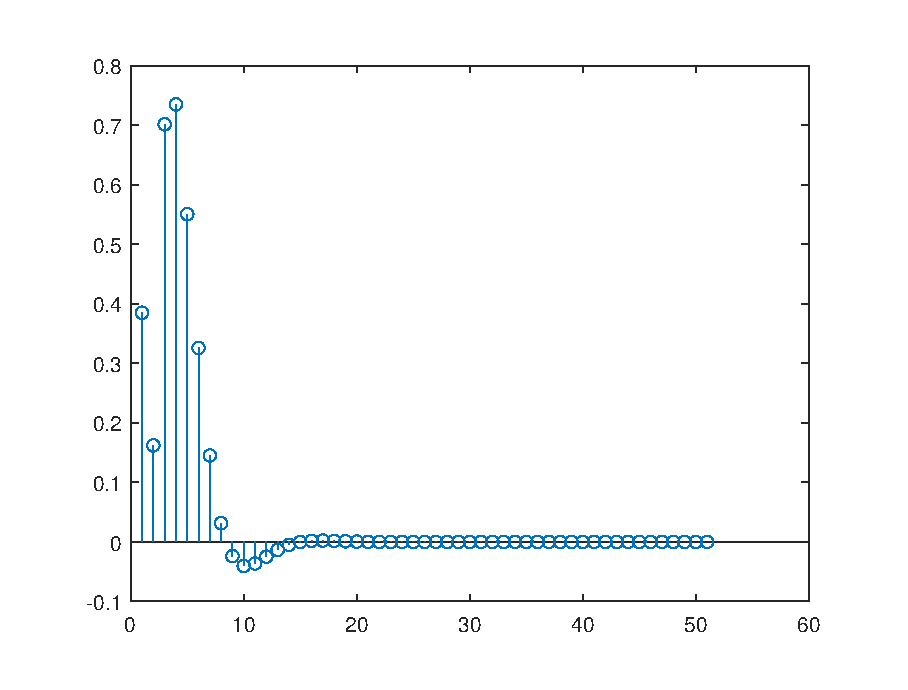
\includegraphics[width=\maxwidth{56.196688409433015em}]{figure_11.eps}
\end{center}
\begin{matlabcode}
figure;
stem(Sresp);
\end{matlabcode}
\begin{center}
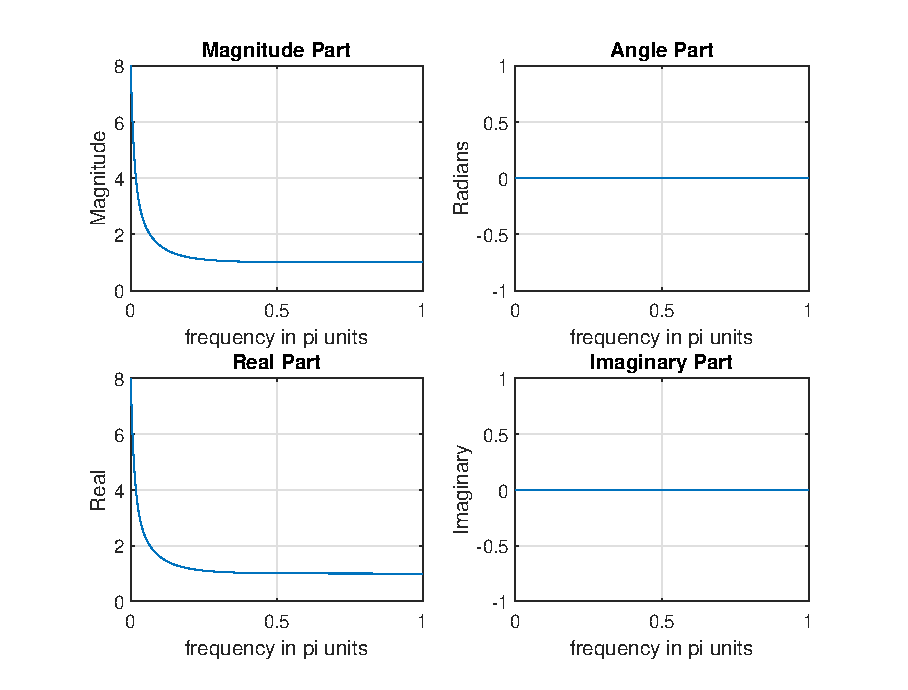
\includegraphics[width=\maxwidth{56.196688409433015em}]{figure_12.eps}
\end{center}

\begin{par}
\begin{flushleft}
Solution 5:
\end{flushleft}
\end{par}

\begin{matlabcode}
%5
n=0:49;
omega=0:pi/49:pi;
h=[ones(1,4)/4  zeros(1,46)];
noisy=exp(j*50*pi/3);
y=conv(noisy,h);
Yw=fft(y);

subplot(2,1,1);
plot(omega,abs(Yw));
subplot(2,1,2);
plot(omega,angle(Yw));
\end{matlabcode}
\begin{center}
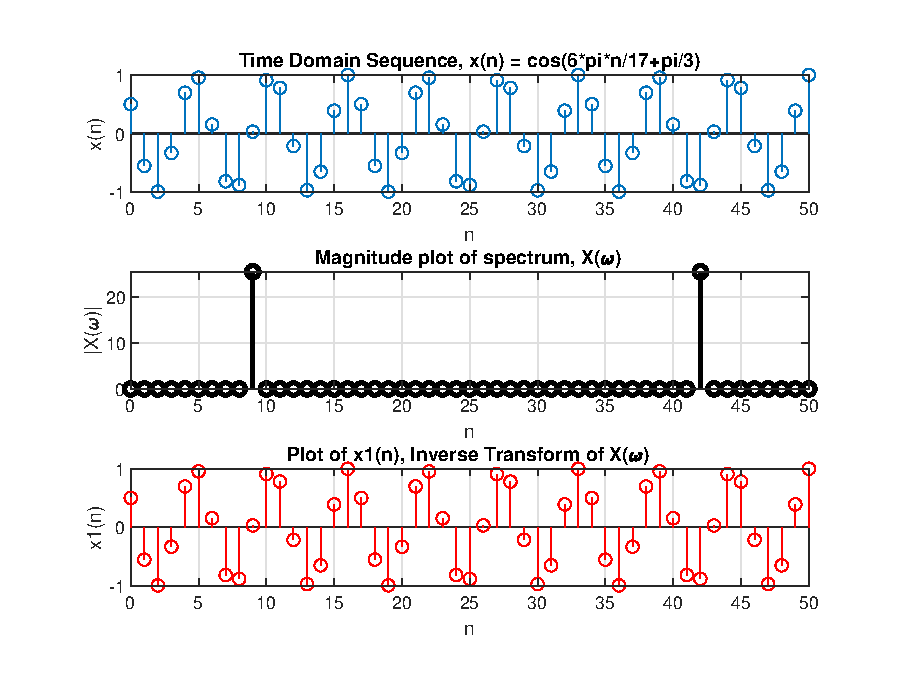
\includegraphics[width=\maxwidth{56.196688409433015em}]{figure_13.eps}
\end{center}

\begin{par}
\begin{flushleft}
Solution 6:
\end{flushleft}
\end{par}

\begin{matlabcode}
%6
\end{matlabcode}

\begin{par}
\begin{flushleft}
Solution 7:
\end{flushleft}
\end{par}

\begin{matlabcode}
%7
n=0:50; 
noisy=cos(6*pi*n/17+pi/3); 
FT=fft(noisy);
xn1=ifft(FT); 
figure; 
stem(n,noisy); 
\end{matlabcode}
\begin{center}
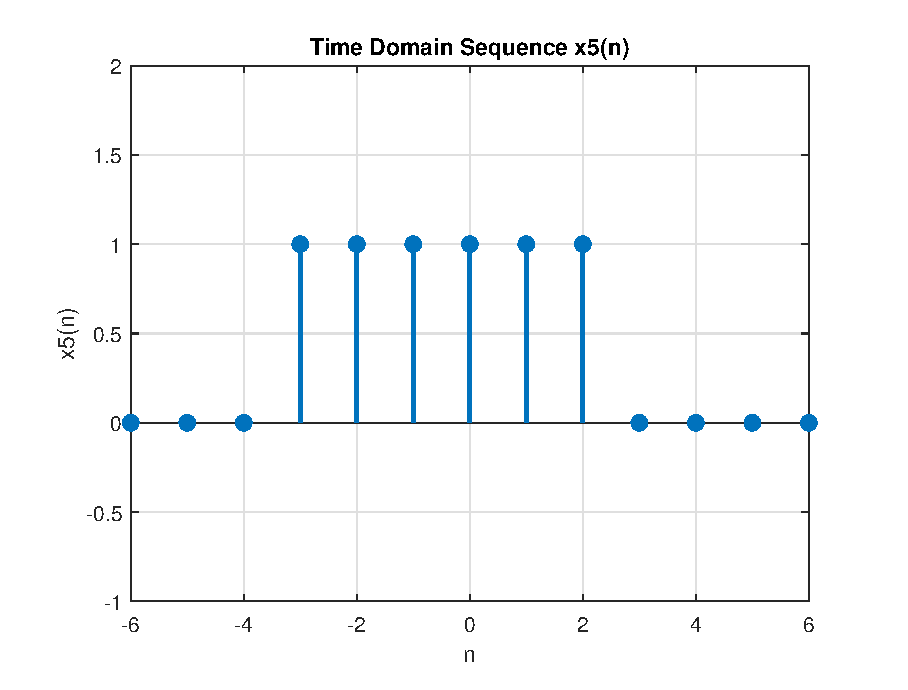
\includegraphics[width=\maxwidth{56.196688409433015em}]{figure_14.eps}
\end{center}
\begin{matlabcode}
figure; 
stem(abs(FT));
\end{matlabcode}
\begin{center}
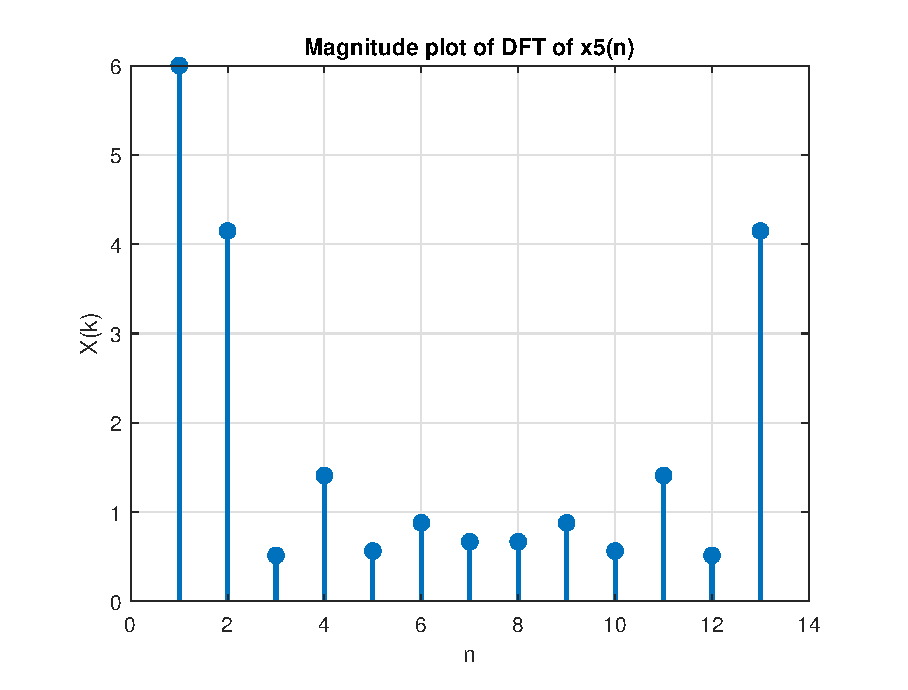
\includegraphics[width=\maxwidth{56.196688409433015em}]{figure_15.eps}
\end{center}
\begin{matlabcode}
figure; 
stem(n,xn1); 
\end{matlabcode}
\begin{center}
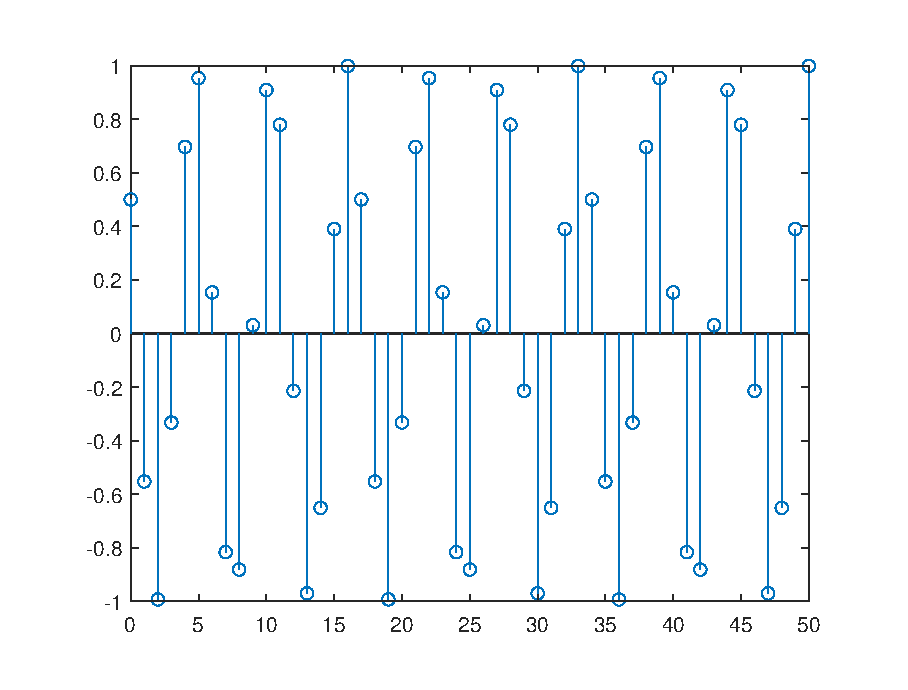
\includegraphics[width=\maxwidth{56.196688409433015em}]{figure_16.eps}
\end{center}

\begin{par}
\begin{flushleft}
Solution 8:
\end{flushleft}
\end{par}

\begin{matlabcode}
%8
n=-6:6; % Indices
x5= [(n+3) >= 0]-[(n-3) >= 0]; % Sequence
D=fft(x5);
figure; 
stem(n,x5);
\end{matlabcode}
\begin{center}
\includegraphics[width=\maxwidth{56.196688409433015em}]{figure_17.eps}
\end{center}
\begin{matlabcode}
figure; 
stem(abs(D));
\end{matlabcode}
\begin{center}
\includegraphics[width=\maxwidth{56.196688409433015em}]{figure_18.eps}
\end{center}
\begin{matlabcode}
figure; 
stem(angle(D));
\end{matlabcode}
\begin{center}
\includegraphics[width=\maxwidth{56.196688409433015em}]{figure_19.eps}
\end{center}

\end{document}
